\documentclass[aspectratio=169,11pt]{beamer}

\IfFileExists{beamerthememetropolis.sty}{%
  \usetheme[numbering=fraction,progressbar=frametitle]{metropolis}
}{%
  \usetheme{CambridgeUS}
  \usecolortheme{dolphin}
}

\usepackage[T1]{fontenc}
\usepackage[utf8]{inputenc}
\usepackage{lmodern}
\usepackage{booktabs}
\usepackage{tabularx}
\usepackage{array}
\usepackage{graphicx}
\usepackage{amsmath}
\usepackage{adjustbox}
\usepackage{tikz}
\usetikzlibrary{arrows.meta,positioning}

\setbeamertemplate{navigation symbols}{}
\setbeamertemplate{footline}[frame number]

\definecolor{zjublue}{RGB}{28,72,116}
\definecolor{zjugray}{RGB}{68,68,68}
\definecolor{lightblue}{RGB}{233,241,248}
\definecolor{lightgreen}{RGB}{232,244,235}
\definecolor{lightred}{RGB}{248,233,232}

\setbeamercolor{frametitle}{fg=white,bg=black!75}
\setbeamercolor{title}{fg=zjublue}
\setbeamercolor{structure}{fg=zjublue}
\setbeamercolor{normal text}{fg=zjugray}
\setbeamercolor{boxblue}{bg=lightblue,fg=zjugray}
\setbeamercolor{boxgreen}{bg=lightgreen,fg=zjugray}
\setbeamercolor{boxred}{bg=lightred,fg=zjugray}
\setbeamerfont{frametitle}{size=\Large,series=\bfseries}
\setbeamerfont{title}{size=\LARGE,series=\bfseries}
\setbeamersize{text margin left=0.65cm,text margin right=0.65cm}
\renewcommand{\arraystretch}{1.18}

\newcommand{\plainbox}[2]{%
  \begin{beamercolorbox}[rounded=true,sep=0.75em,wd=\textwidth]{#1}
    #2
  \end{beamercolorbox}
}

\begin{document}

% Slide 1
\begin{frame}[plain]
  \vspace{0.55cm}
  {\usebeamerfont{title}\usebeamercolor[fg]{title}
  When Do China's Critical-Mineral\\Export Controls Bind?\par}
  \vspace{0.35cm}
  {\large Evidence from Graphite, Gallium--Germanium, and Antimony\par}
  \vfill
  {\large Mario D. Martinez\par}
  \vspace{0.12cm}
  {Master in Chinese Economy -- Zhejiang University\par}
  {Course: Introduction to China's Foreign Trade and Investment\par}
  \vspace{0.25cm}
  {June 17, 2026\par}
\end{frame}

% Slide 2
\begin{frame}{Roadmap}
  \large
  \begin{enumerate}
    \item Why licensing controls may or may not matter
    \item Research question and intuition
    \item Data and empirical model
    \item Main results
    \item What the results imply
  \end{enumerate}
\end{frame}

% Slide 3
\begin{frame}{Motivation: Licensing Is Not a Ban}
  \large
  \begin{itemize}
    \item ``Controlled'' = covered by China's export-license rule.
    \item A license is not an automatic export ban.
    \item It can create delays, paperwork, uncertainty, or denial risk.
    \item So the empirical question is: did imports from China fall?
  \end{itemize}

  \vspace{0.35cm}
  \begin{center}
  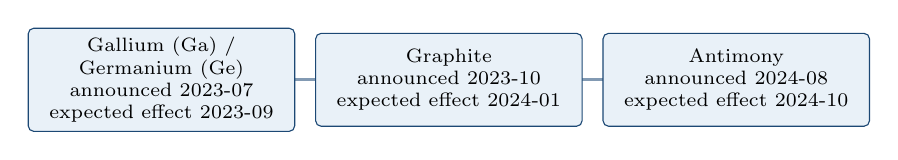
\begin{tikzpicture}[
    x=1cm,y=1cm,
    event/.style={draw=zjublue,fill=lightblue,rounded corners=2pt,
      align=center,text width=3.15cm,minimum width=3.15cm,minimum height=1.18cm,font=\scriptsize}
  ]
    \draw[very thick,zjublue!55] (0,0) -- (10.4,0);
    \node[event] at (1.55,0) {Gallium (Ga) /\\Germanium (Ge)\\announced 2023-07\\expected effect 2023-09};
    \node[event] at (5.2,0) {Graphite\\announced 2023-10\\expected effect 2024-01};
    \node[event] at (8.85,0) {Antimony\\announced 2024-08\\expected effect 2024-10};
  \end{tikzpicture}
  \end{center}
\end{frame}

% Slide 4
\begin{frame}{Research Question}
  \large
  \textbf{When do China's licensing-based controls reduce importers' reliance on China?}

  \vspace{0.25cm}
  \begin{center}
  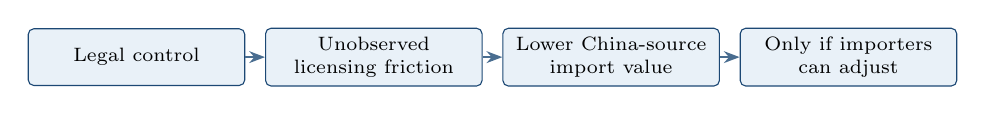
\begin{tikzpicture}[
    node distance=0.25cm,
    flowbox/.style={draw=zjublue,fill=lightblue,rounded corners=2pt,
      align=center,minimum width=2.75cm,minimum height=0.72cm,font=\scriptsize},
    arr/.style={-{Stealth[length=2mm]},thick,zjublue!80}
  ]
    \node[flowbox] (a) {Legal control};
    \node[flowbox,right=of a] (b) {Unobserved\\licensing friction};
    \node[flowbox,right=of b] (c) {Lower China-source\\import value};
    \node[flowbox,right=of c] (d) {Only if importers\\can adjust};
    \draw[arr] (a) -- (b);
    \draw[arr] (b) -- (c);
    \draw[arr] (c) -- (d);
  \end{tikzpicture}
  \end{center}

  \vspace{0.08cm}
  \begin{beamercolorbox}[rounded=true,sep=0.55em,wd=\textwidth]{boxblue}
    \scriptsize Unobserved licensing friction = delay, paperwork, uncertainty, denial risk, or higher cost from the license process.
  \end{beamercolorbox}

  \vspace{0.08cm}
  \scriptsize I cannot observe the friction directly. I test whether trade values move as if buying from China became harder.

  \vspace{0.04cm}
  \scriptsize
  \begin{itemize}
    \item China exposure = pre-control reliance on China.
    \item Adjustment capacity = existing non-China supplier links.
    \item Product scope = how cleanly the rule maps to the trade code.
  \end{itemize}

  \vspace{-0.05cm}
  \plainbox{boxblue}{\small A legal control is binding in the data only if trade flows actually move.}
\end{frame}

% Slide 5
\begin{frame}{Data: What the Model Sees}
  \small
  \begin{tabularx}{\textwidth}{>{\bfseries}p{0.22\textwidth}X}
    \toprule
    Dimension & What it means \\
    \midrule
    Time & Monthly, 2019-01 to 2026-03 \\
    Countries & 53 reporting importers \\
    Products & 10 Harmonized System (HS) product headings \\
    Source & China vs Rest of World (ROW) \\
    Outcome & Monthly import value in USD \\
    Controls & Alumina, manganese articles, inorganic acids \\
    \bottomrule
  \end{tabularx}

  \vspace{0.18cm}
  \small ROW = Rest of World = all non-China suppliers.

  \vspace{0.22cm}
  \plainbox{boxblue}{%
    \normalsize One observation: importer \(i\) buys product \(p\) from source \(s\) in month \(t\).

    \vspace{0.12cm}
    \small Example: Germany imports HS 282580 (Antimony oxides) from China in Nov. 2024.
  }
\end{frame}

% Slide 6
\begin{frame}{Empirical Model: What Is Being Compared?}
  \vspace{-0.25cm}
  \scriptsize
  \[
  \begin{aligned}
  \mathbb{E}[M_{ipst}\mid X]
  &=
  \exp\left[
  \beta\left(Treated_p \times China_s \times Post_{pt}\right) \right.\\
  &\quad \left.
  +\alpha_{ip}+\alpha_{is}+\alpha_{pt}
  +\alpha_{st}+\alpha_{ps}+\alpha_{it}
  \right]
  \end{aligned}
  \]

  \vspace{-0.35cm}
  {\tiny \(X\) summarizes the fixed effects and variables shown in the model.}

  \vspace{-0.25cm}
  \begin{columns}[T,totalwidth=\textwidth]
    \begin{column}{0.47\textwidth}
      \centering
      \[
      \Downarrow \quad \text{Simply:}
      \]
      \vspace{-0.25cm}
      \[
      Treated\ product \times China\ source \times After\ policy
      \]

      \begin{beamercolorbox}[rounded=true,sep=0.50em,wd=\textwidth]{boxblue}
        \footnotesize I compare: treated vs untreated products; China vs ROW sources; after vs before the control.
      \end{beamercolorbox}
    \end{column}
    \begin{column}{0.49\textwidth}
      \scriptsize
      \begin{tabularx}{\textwidth}{>{\bfseries}p{0.24\textwidth}X}
        \(M_{ipst}\) & monthly import value \\
        \(i,p,s,t\) & importer, product, source, month \\
        \(Treated_p\) & product covered by licensing rule \\
        \(China_s\) & source is China \\
        \(Post_{pt}\) & after product \(p\)'s expected import-effect month \\
        \(\beta\) & relative China-source import-value change \\
        \(\alpha\)'s & fixed effects for normal country, product, source, and month differences \\
      \end{tabularx}
    \end{column}
  \end{columns}
\end{frame}

% Slide 7
\begin{frame}{Why PPML?}
  \large
  \begin{itemize}
    \item Many trade flows are zero.
    \item Trade values are very uneven.
    \item PPML keeps zero trade flows in the data.
    \item The coefficient can be reported as a percent effect.
  \end{itemize}

  \vspace{0.35cm}
  \plainbox{boxblue}{%
    \large PPML = Poisson pseudo-maximum likelihood. Even though the name sounds like counts, here PPML models trade values.
  }

  \vspace{0.25cm}
  \large
  Example: if \(\beta=-1.69\), then \(100(e^{-1.69}-1)\approx -81.5\%\).
\end{frame}

% Slide 8
\begin{frame}{Product-Level Results: Effects Are Selective}
  \scriptsize
  Gallium = Ga; Germanium = Ge; Zirconium = Zr. Pretrend = whether treated and comparison flows moved similarly before the control.

  \vspace{0.08cm}
  \renewcommand{\arraystretch}{1.06}
  \begin{adjustbox}{max width=\textwidth}
  \begin{tabular}{p{0.40\textwidth}rccp{0.24\textwidth}}
    \toprule
    Product & Effect & Reporter \(p\) & Pretrend? & Interpretation \\
    \midrule
    HS 282580 (Antimony oxides) & \(-81.5\%\) & 0.002 & OK & clean central case \\
    HS 8110 (Antimony metal) & \(-86.8\%\) & \(<0.001\) & fails & consistent, not clean \\
    HS 261710 (Antimony ores) & \(-98.9\%\) & 0.003 & fails/sparse & descriptive only \\
    HS 2504 (Natural graphite) & \(-30.4\%\) & 0.107 & fails & suggestive \\
    HS 811292 (Ga/Ge-containing bundle) & \(+19.3\%\) & 0.365 & fails & no aggregate negative effect \\
    HS 282560 (GeO$_2$/ZrO$_2$) & \(+17.5\%\) & 0.271 & OK & no aggregate negative effect \\
    \bottomrule
  \end{tabular}
  \end{adjustbox}
  \renewcommand{\arraystretch}{1.18}

  \vspace{0.15cm}
  \scriptsize
  Reporter \(p\)-values are diagnostics. Exact product-assignment \(p\)-value floor = 0.25.
\end{frame}

% Slide 9
\begin{frame}{Central Case: HS 282580 (Antimony Oxides)}
  \begin{columns}[T,totalwidth=\textwidth]
    \begin{column}{0.62\textwidth}
      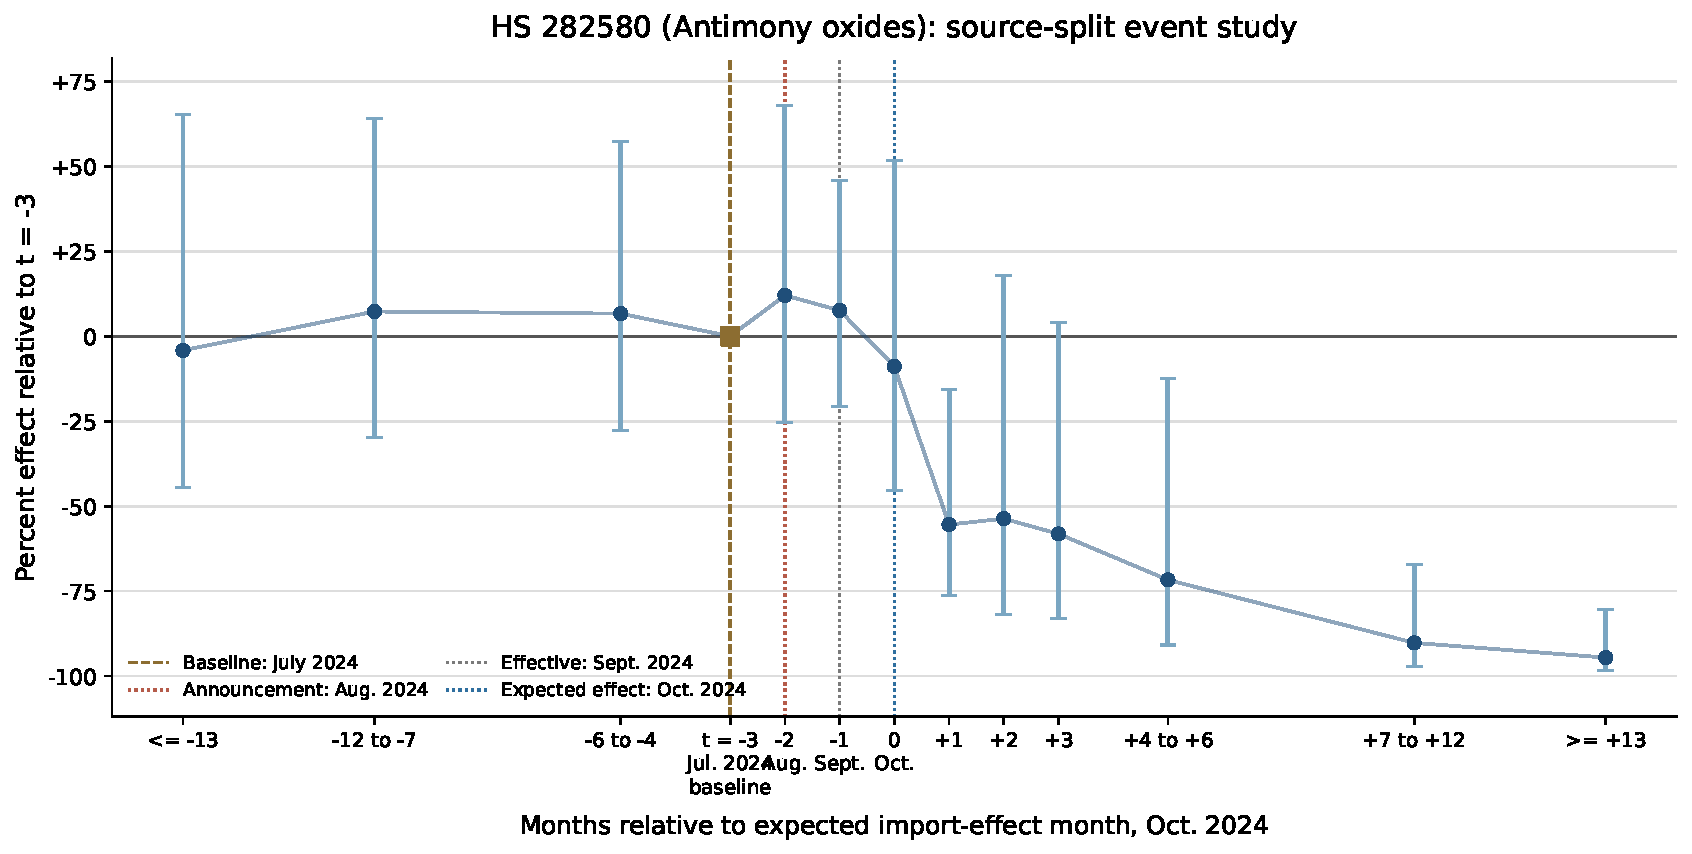
\includegraphics[width=\textwidth]{figures/hs282580_eventstudy_slides.pdf}
    \end{column}
    \begin{column}{0.35\textwidth}
      \small
      \begin{itemize}
        \item Static effect: \(-81.5\%\).
        \item Pretrend \(p=0.680\).
        \item Evidence consistent with binding licensing friction.
      \end{itemize}

      \vspace{0.08cm}
      \begin{beamercolorbox}[rounded=true,sep=0.55em,wd=\textwidth]{boxblue}
        \scriptsize \(t=0\): Oct. 2024 expected effect. \(t=-1\): Sept. effective date. \(t=-2\): Aug. announcement. \(t=-3\): July 2024, last clean pre-announcement month.
      \end{beamercolorbox}

      \vspace{0.06cm}
      \scriptsize \textbf{Down = less China-source import value} relative to ROW and controls.
    \end{column}
  \end{columns}
\end{frame}

% Slide 10
\begin{frame}{HS 282580: Who Adjusts?}
  \scriptsize
  \textit{Switching potential is measured before the antimony control.}

  \vspace{-0.04cm}
  For each importer-product pair, I calculate:

  \vspace{-0.22cm}
  \[
  A_{ik}=\text{China exposure}_{ik}\times \text{ROW access}_{ik}
  \]

  \vspace{-0.30cm}
  \scriptsize
  \begin{itemize}
    \item \(i\) = importing country; \(k\) = product.
    \item China exposure = pre-control share of imports from China.
    \item ROW access = share of pre-control months with any non-China import.
    \item High \(A_{ik}\) = dependent on China but already connected to other suppliers.
  \end{itemize}

  \vspace{0.04cm}
  Then I split importers into high vs low \(A_{ik}\) and re-run the same model for HS 282580 (Antimony oxides).

  \vspace{0.08cm}
  \begin{columns}[T,totalwidth=\textwidth]
    \begin{column}{0.48\textwidth}
      \begin{beamercolorbox}[rounded=true,sep=0.42em,wd=\textwidth]{boxgreen}
        \small\textbf{High switching potential importers}

        \vspace{0.04cm}
        {\Large Model effect: \(-87.4\%\)}

        \vspace{0.04cm}
        \scriptsize China-source import value falls strongly.
      \end{beamercolorbox}
    \end{column}
    \begin{column}{0.48\textwidth}
      \begin{beamercolorbox}[rounded=true,sep=0.42em,wd=\textwidth]{boxred}
        \small\textbf{Low switching potential importers}

        \vspace{0.04cm}
        {\Large Model effect: \(+103.1\%\)}

        \vspace{0.04cm}
        \scriptsize No China-source decline.
      \end{beamercolorbox}
    \end{column}
  \end{columns}

  \vspace{0.06cm}
  \scriptsize These are relative PPML effects for HS 282580 (Antimony oxides) only, not simple before/after averages.

  \begin{beamercolorbox}[rounded=true,sep=0.35em,wd=\textwidth]{boxblue}
    \scriptsize The decline appears where importers both needed to adjust and had alternative suppliers. This supports a source-switching interpretation for antimony oxides.
  \end{beamercolorbox}
\end{frame}

% Slide 11
\begin{frame}{What Should We Learn?}
  \large
  \begin{itemize}
    \item A legal control is not automatically a trade disruption.
    \item Countries with non-China suppliers can shift sourcing more easily.
    \item HS product codes can mix controlled and uncontrolled items.
    \item Do not assume every product in one announcement behaves the same.
    \item Value data cannot separate prices, quantities, rerouting, or demand.
  \end{itemize}

  \vfill
  \plainbox{boxblue}{\large Main message: one clean product effect, several caveated or null cases.}
\end{frame}

\appendix

% Slide 12
\begin{frame}[noframenumbering]{Key References}
  \large
  \begin{itemize}
    \item MOFCOM/GAC announcements: legal dates and product scope.
    \item UN Comtrade: monthly bilateral import data.
    \item IEA / USGS: mineral concentration background.
    \item Farrell \& Newman: chokepoints and interdependence.
    \item Bown / Bown \& Wang: U.S.--China technology conflict.
    \item Roth: event-study and pretrend inference caution.
  \end{itemize}
\end{frame}

\end{document}
